\documentclass[12pt,a4paper]{article}
\usepackage[utf8]{inputenc}
\usepackage{amsmath}
\usepackage{amsfonts}
\usepackage{amssymb}
\usepackage{listings}
\usepackage{url}
\usepackage[bulgarian]{babel}
\usepackage{listings}
\usepackage{enumerate}
\usepackage{graphicx}
\usepackage{relsize}


\lstset{breaklines=true} 


\author{\textit{email: kalin@fmi.uni-sofia.bg}}
\title{\textsc{Задачи за задължителна самоподготовка} \\
по \\
Увод в програмирането\\
\textit{Рекурсия с връщане назад}}



\begin{document}
\maketitle

\begin{flushleft}
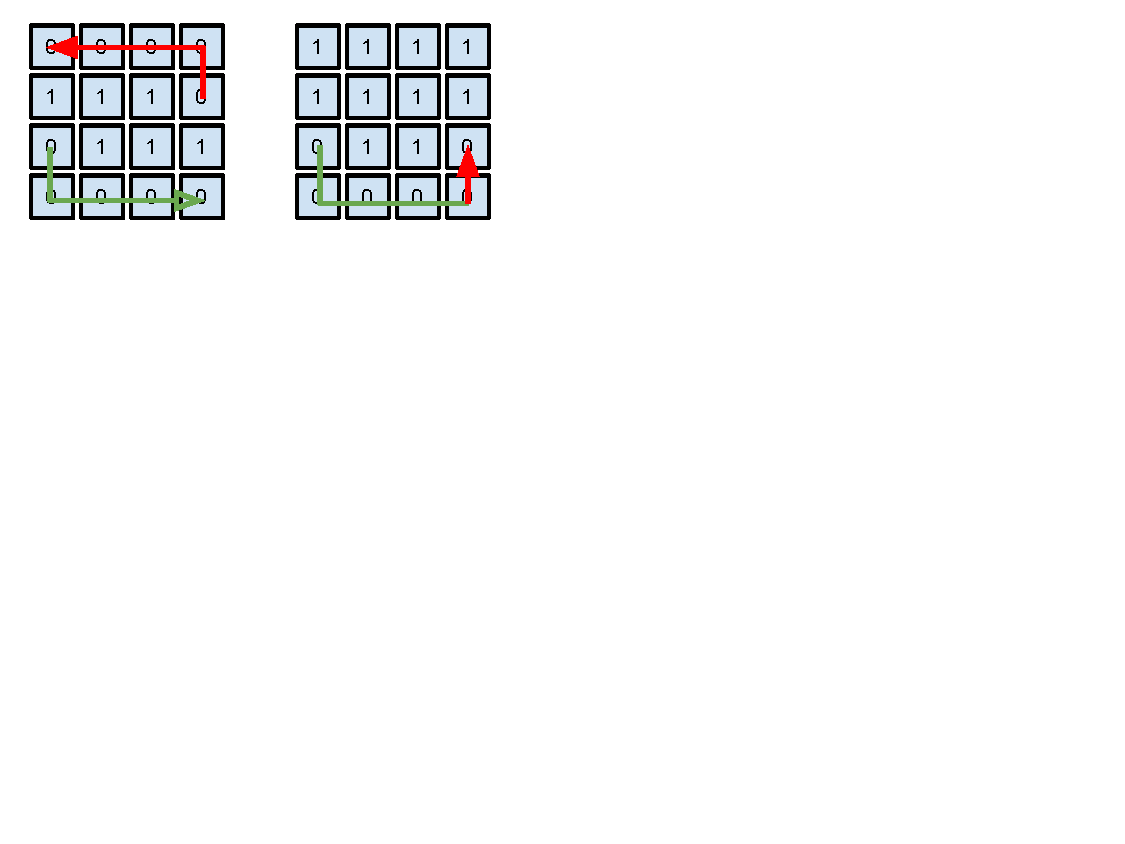
\includegraphics[width=15cm]{images/path1}

\vspace{-200px}

\relscale{0.8}
Фигура 1a и 1б. Примерени лабиринти
\end{flushleft}


\begin{enumerate}
	
	\item Нека е дадена квадратна матрица от цели числа $N \times N$, представяща ``лабиринт''. Елементи на матрицата със стойност $0$ смятаме за ``проходими'', а всички останали - за ``непроходими''. Път в лабиринта наричаме всяка последователност от проходими елементи на матрицата, които са съседни вертикално или хоризонтално, такава че (1) никой елемент от последователноста не е последван директно от предшественика си (забранено е ``връщането назад'') и (2) най-много един елемент на последователноста се среща в нея повече от веднъж (има най-много един ``цикъл'').

	Да се дефинира функция \texttt{bool downstairs (int sx, int sy, int tx, int ty)}, която проверява дали съществува път от елемента $(sx,sy)$ до елемента $(tx,ty)$, такъв, че всеки следващ елемент от пътя е или вдясно, или под предишния. Такъв път да наричаме ``низходящ''. 

	Пример: На фигура 1a такъв път съществува от елемента $(0,2)$ до елемента $(3,3)$, но не и от $(3,1)$ до $(0,0)$.

	\item При условията на дефинициите от предишната задача, да се дефинира функция \texttt{bool connected()}, която проверява дали от всеки елемент на матрицата $(sx,sy)$ до всеки елемент на матрицата  $(tx,ty)$, такива, че $sx \leq tx$ и $sy \leq ty$, съществува низходящ път. 

	Пример: За лабиринта от фиг. 1a условието е изпълнено, но не и за лабиринта от фигура 1б.


	\item Да се напише програма, която по въведени от клавиатурата $4 \le n \le 8$ и $0 \le k \le n$ намира извежда на екрана всички възможни конфигурации на абстрактна шахматна дъска с размери $n \times n$ с разположени на нея $k$ коня така, че никоя фигура не е поставена на поле, което се ``бие'' от друга фигура според съответните шахматни правила. 

	Пример за отпечатана конфигурация с $n=5, k=2$:
	\begin{verbatim}
	_ _ _ _ _
	_ _ R _ _
	_ _ _ _ _
	_ _ _ _ R
	_ _ _ _ _
		
	\end{verbatim}


	\item При условията на първа задача да се напише функция

	\texttt{int minDistance (int sx, int sy, int tx, int ty)},

	която по въведени от клавиатурата координати на елементи $s=(sx,sy)$ и $t=(tx,ty)$ намира \textit {дължината} на най-краткия път между $s$ и $t$. Обърнете внимание, че се иска \textit{път}, а не просто низходящ път.

	\item 

	При условията на първа задача да се напише функция, която по въведени от клавиатурата координати на елементи $s=(sx,sy)$ и $t=(tx,ty)$ намира и отпечатва на екрана елементите, от които се състои най-краткия път между $s$ и $t$. Обърнете внимание, че се иска \textit{път}, а не просто низходящ път.


	\item Пъзел на Синди\cite{cindy}.

	Дадена е игрова дъска като на фигура 2, която се състои от $n$ черни и $n$ бели фигури. Фигурите могат да бъдат разположени на $2n+1$ различни позиции. Играта започва с разполагане на всички черни фигури вляво, а всички бели - вдясно на дъската.

	Черните фигури могат да се местят само надясно, а белите - само наляво. На всеки ход важат следните правила:


	\begin{itemize}
		\item всяка фигура се мести само с по една позиция, ако съответната позиция не е заета;
		\item ако позицията е заета, фигурата $X$ може да прескочи точно една фигура $Y$ от противоположния цвят, ако позицията след $Y$ e свободна.
	\end{itemize}

	Да се напише програма, която по въведено число $n$ отпечатва на екрана инструкции за игра така, че в края на играта всички бели фигури да са вляво на дъската, а всички черни - вдясно. Инструкциите да са от следния вид:

	\begin{verbatim}
		Прместете бяла фигура от позиция 5 на позиция 3.
	\end{verbatim}

	На следните фигури е даден пример за игра:

	\begin{flushleft}
	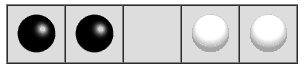
\includegraphics[width=5cm]{images/step0}

	\relscale{0.8}
	1. Начална конфигурация.
	\end{flushleft}


	\begin{flushleft}
	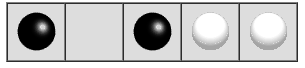
\includegraphics[width=5cm]{images/step1}

	\relscale{0.8}
	2. Преместване на черна фигура с един ход надясно.
	\end{flushleft}

	\begin{flushleft}
	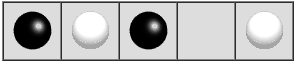
\includegraphics[width=5cm]{images/step2}

	\relscale{0.8}
	3. Преместване на бяла фигура с прескачане.
	\end{flushleft}

	\begin{flushleft}
	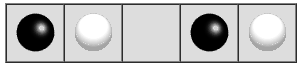
\includegraphics[width=5cm]{images/step3}

	\relscale{0.8}
	4. Преместване на черна фигура с един ход надясно.
	\end{flushleft}

	\begin{flushleft}
	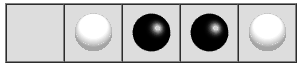
\includegraphics[width=5cm]{images/step4}

	\relscale{0.8}
	5. Преместване на черна фигура чрез прескачане
	\end{flushleft}

	След ход 5 конфигурацията на играта е безперспективна.


\end{enumerate}


	\vspace{20px}

	\small{Някои от задачите са от сборника \textit{Магдалина Тодорова, Петър Армянов, Дафина Петкова, Калин Николов, ``Сборник от задачи по програмиране на C++. Първа част. Увод в програмирането''}. За тези задачи е запазена номерацията в сборника.}

\begin{thebibliography}{99}

\bibitem{cindy}	David Matuszek, ``Backtracking'', https://www.cis.upenn.edu/~matuszek/cit594-2012/Pages/backtracking.html.

\end{thebibliography}

\end{document}

